\section*{Properties of IVPU game}
Like the above, divide the characteristic function into two parts like $c(s,P) = c_0(s,m^*(s)) + P\cdot m^*(s), s \in S$.

As a common practice, we can obtain the dual of $\omega(P)$:

\begin{equation}\label{dual}
 {\omega^*(P)}=\mathop{\max}_{\rho} \{c_0(V)+m(V)P+\sum_{s\in S}-\rho_s[c_0(s,m^*(s)) + P\cdot m^*(s)]:
 \sum_{s\in S:k\in s}\rho_s=1,\forall k \in V,\rho_s\geq 0,\forall s \in S \}
\end{equation}

By deriving $\omega^*(P)$ with respect to $P$, we can obtain lemma \ref{lem1}.

\begin{lem}\label{lem1}
The sum of absolute values of slopes at both sides of $P_i$ is 1.
\end{lem}

Based on the above defined PSPF, we can establish Theorem \ref{thm2} below, showing the property of this function.

\begin{thm}\label{thm2}
$\omega(P)$ is piecewise linear, and convex in price P at each sub-interval $[P_{i+1},P_{i}], i \in \{1,2,\ldots,v-1\}$.
\end{thm}

In this situation, the size of interval $I_i$ can be calculated when $t_i,i \in \{1,2,\ldots,v\}$ is known. As shown previously, the extreme points of these intervals are recorded as $P_i$ respectively, which represents the price when the number of using machine changes from $i$ to $i-1$. Specially, $P_1$ denotes the right extreme point of the whole interval, which is the value of price when using one machine and subsidy equals zero.

Note that the costs of all the exponential coalitions can be easily calculated by the SPT rules, we have lemma \ref{lem2}.

\begin{lem}\label{lem2}
The breaking price, $P_i(2 \leq i \leq v)$, which is at the extreme points of the sub-intervals $I_i$ can be obtained by SPT rules in polynomial time.
\end{lem}

According to the above lemma \ref{lem2}, we can obtain all the extreme points of the sub-intervals $P_i, 2 \leq i \leq v$. When the price increase from $P_i^-$(little smaller than $P_i$) to $P_i^+$(little larger than $P_i$), the number of machines used by the grand coalition will decrease one.

\begin{thm}\label{thm3}
Boundary price $P^*$ or $P_1$ equals $\sum_{i=2}^v P_i$, and can be obtained in polynomial time.
\end{thm}

With theorem \ref{thm3}, we obtain all the breakpoints during the whole price interval $[0,P^*]$. Then we'll focus on the specific property of subsidy.

\begin{thm}\label{thm4}
$\omega(P)$ can be bounded by zero when the number of machines used by the grand coalition $V$ is larger than $\frac{v}{2}$.
\end{thm}

In other words, when the number of machines used is larger than half of players, the grand coalition doesnot need any subsidy from the externality.

Define a new game, that is Single Machine Scheduling Game(SMSG)
\[
\begin{aligned}
c(s,P,'m='1) = & {\min} \sum_{k\in V}\sum_{j\in O} {c_{kj} x_{kj} + P} \\
{s.t.}\quad & \sum_{j \in O} x_{kj}-y_k^s=0, \forall k \in V, \\
& \sum_{k\in V} x_{kj} \leq 1, \forall j \in O,  \\
& x_{kj} \in \{0,1\} , \forall k \in V, \forall j \in O,\\
& y_k^s=1, k \in s, y_k^s=0, k \notin s.
\end{aligned}
\]

\begin{thm}\label{thm5}
For SMSG(or, MSG with only one machine), given $P \in [P_2, P^*]$ (or, $[P_2,P_1]$),
the slope range of each segments in the interval for function $\omega(P)$ is within $\left(-1, -\frac{1}{n-1} \right]$, and the number of breakpoints in the same interval for function $\omega(P)$ is within $O(v^2)$.
\end{thm}

Until here, we described the main property of the whole figure.
And a diagram of the number of machines used and subsidy on price with essential features is showed below.

\begin{figure}[h]%%图
	\centering  %插入的图片居中表示
	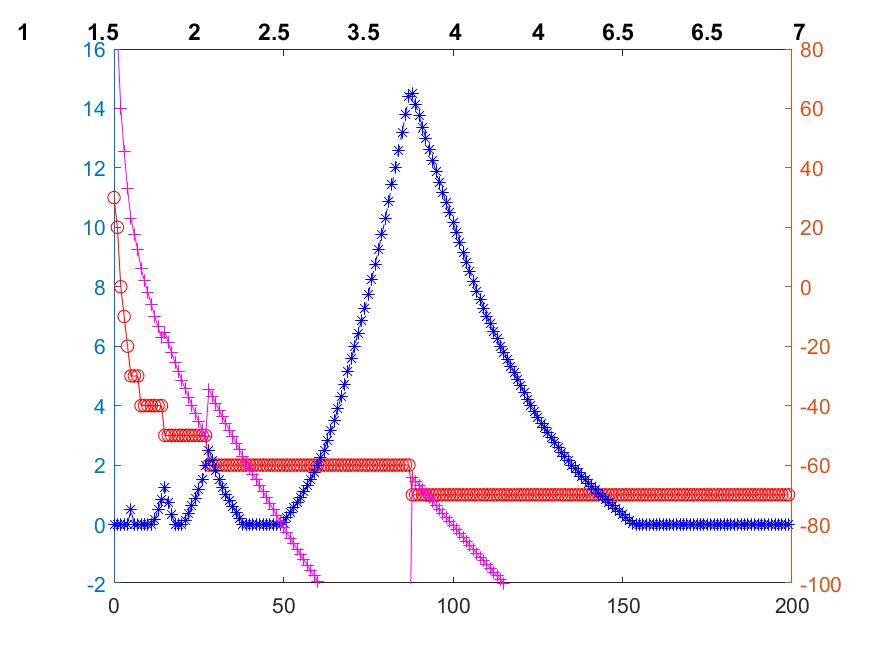
\includegraphics[width=0.8\linewidth]{Figures/Image30}  %插入的图,包括JPG,PNG,PDF,EPS等,放在源文件目录下
	\caption{The number of machines and subsidy on setup cost.}  %图片的名称
	\label{fig:Image11}   %标签,用作引用
\end{figure}

\begin{remark}
  When the number of available machines $m$ is larger than $v$, the image is complete, just like the above shown. However, when the number of available machines $m$ is less than $v$, the image will be truncated, which means the corresponding part of the price less than $P_{m+1}$ should be removed from the figure. While the properties of the rest part will still hold.
\end{remark}

The processing times of all jobs with the arrangement from small to large are listed on the top of this figure.
The red and blue lines stand for the machine number and subsidy, respectively.
The horizontal ordinate represents the price.
The left ordinate represents the number of machine used, while the right represents the value of subsidy.

Compared with the traditional characteristic function $c(s)$, characteristic function defined in the IVPU game has another parameter, the number of machines used by coalition $m(s)$, whose exponential numbers of $m(s)$ bring more difficulties to the solution.
In order to address this problem, we establish the Theorem \ref{thm5}.

\begin{thm}\label{thm5}
  Define that
  \[
    {\omega_1(P)}=\mathop{\min}_{\alpha}\{c(V,P)-\alpha(V): \alpha(s)\leq c(s,P,1), \forall s \in S, \alpha\in\mathbb{R}^{v}\},
  \]
then the original problem $\omega(P)$ is equivalent to $\omega_1(P)$.
\end{thm}

As the coalitional stability constraints showed above, the exponential inequality constraints are so tricky that we must figure out a method to eliminate redundant constraints to obtain the optimal results.

With the Theorem 5, which will save us from the trouble of solving $c(s, P)$ and speed up the solution, we can use the cutting plane method to eliminate the redundant inequalitie, then  any value of $\omega_1(P)$ can be polynomially solvable when given $P$.
